\documentclass[compress]{beamer}
\usepackage[ngerman]{babel}
\usepackage{graphicx}
\usepackage{subfiles}
\usepackage{listings}

\graphicspath{{resources/}}

\setbeameroption{show notes}

\usetheme[noflama]{custom}

\title{Funktionale \break Programierung}
\subtitle{Nebenläufigkeit \& Parallelisierung}
\author{Jan-Philipp Willem}
\institute{Prof. Dr. Sandro Leuchter\\
  Fakultät für Informatik\\
  Hochschule Mannheim
}
\date{Seminar, WS2016}

\begin{document}

\begin{frame}[noframenumbering,plain]
  \frametitle{Was wird hier gezeigt?}
  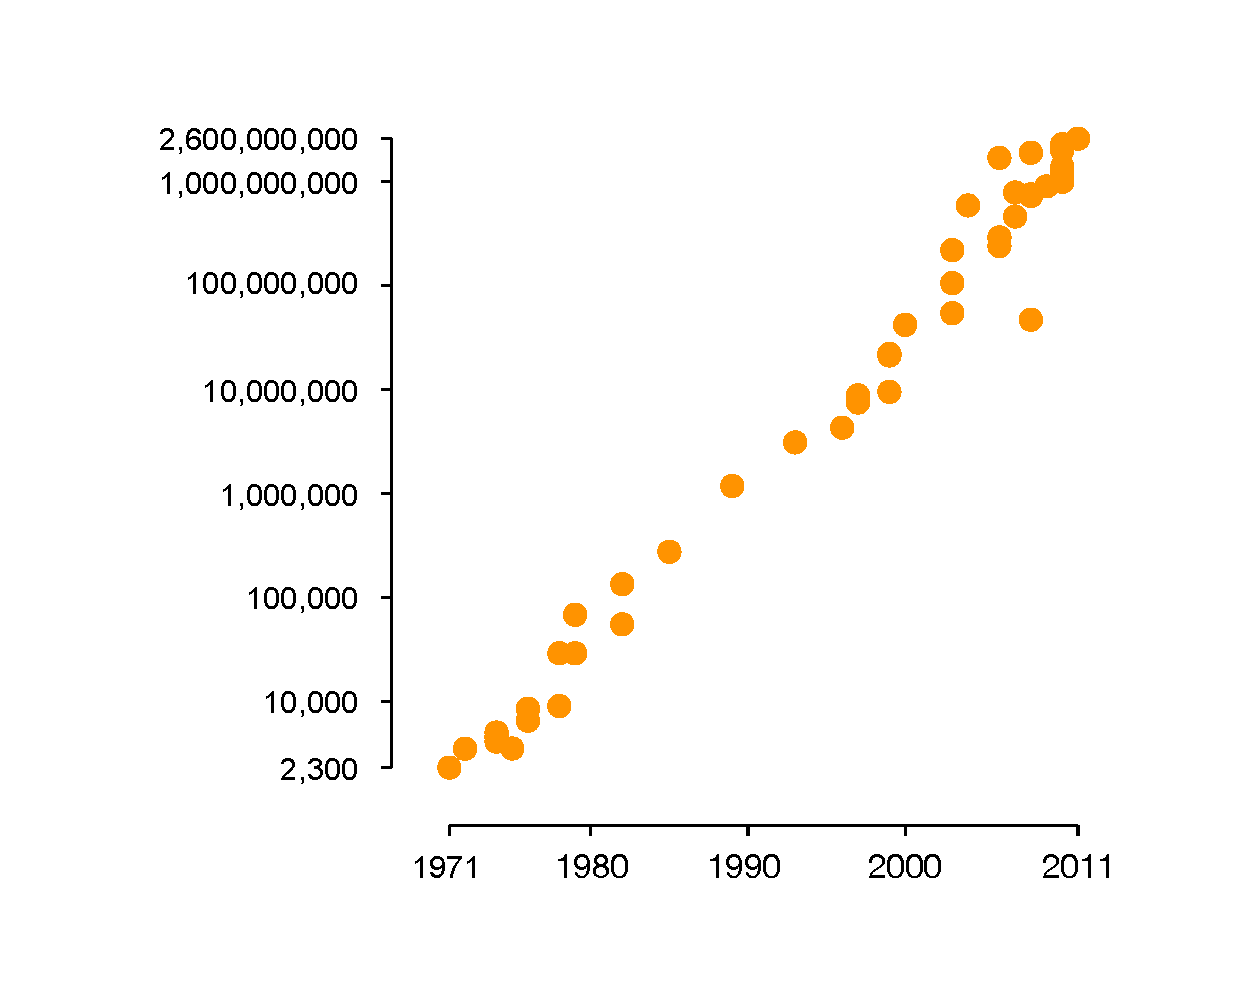
\includegraphics[width=0.9\textwidth]{moores_law.pdf}
\end{frame}

\begin{frame}[noframenumbering,plain]
  \frametitle{Transistor Counts 1971-2011 \& Moore's Law}
  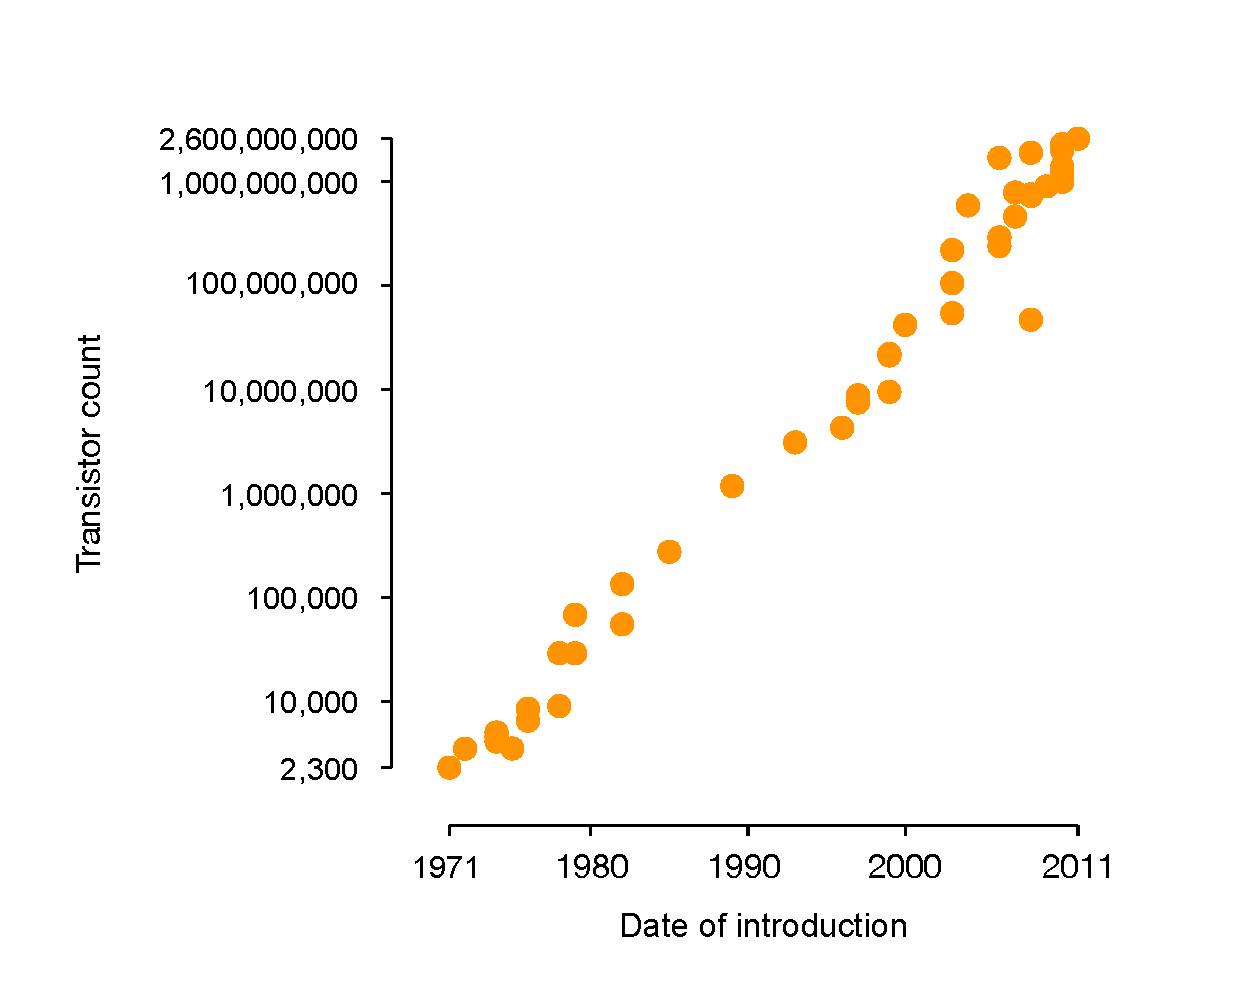
\includegraphics[width=0.9\textwidth]{moores_law_with-labels.pdf}
\end{frame}
  
  \note[itemize]{
     \item relation von transitor anzahl und deren produkt-release
     \item man sieht augenscheinlich, dass sich die anzahl jeweilig verdoppelt hat
     \item viele vermuten, dass sich die moore's law bewahrheitet hat
     \item man munkelt, dass wir damit nun allmählich an die grenzen gelangt sind
  }

\begin{frame}[noframenumbering,plain]{arsTECHNICA UK - 03.01.2017 (1)}
  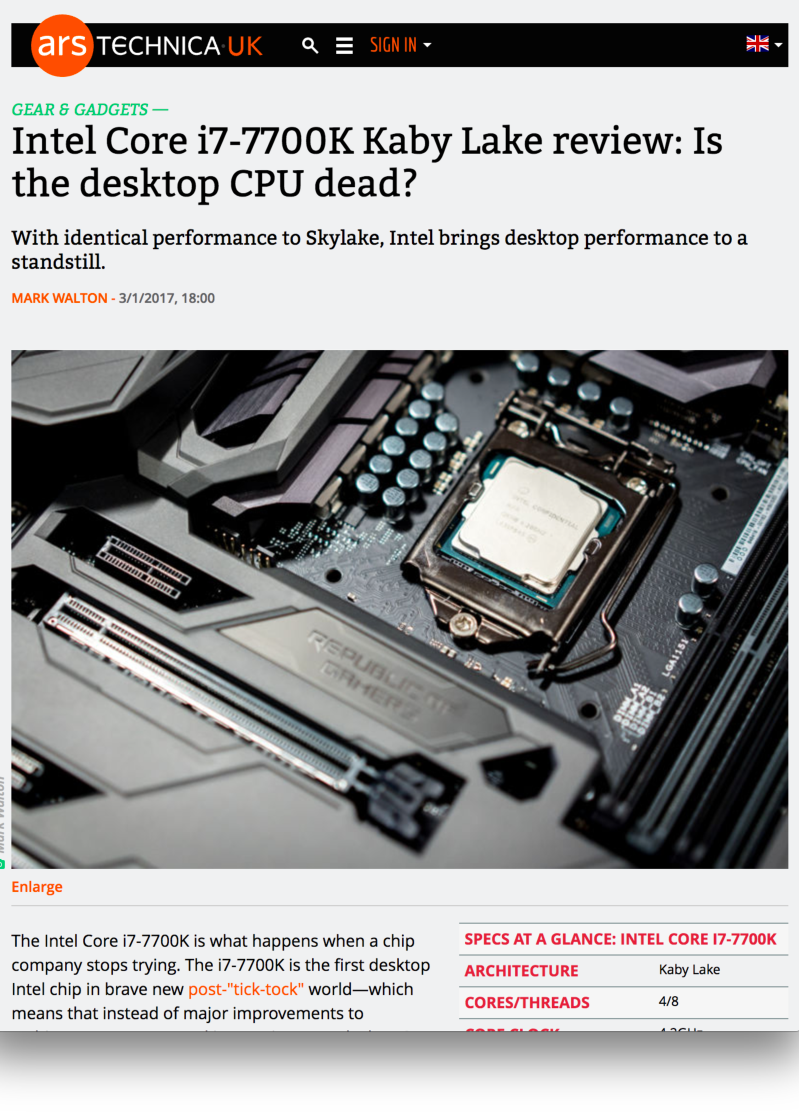
\includegraphics[width=\textwidth]{news.pdf}
\end{frame}

% \begin{frame}[noframenumbering,plain]{arsTECHNICA UK - 03.01.2017 (2)}
%   „[...] With low-power laptops and all-in-ones continuing to outsell desktops—and with high-end workloads like video editing, 3D animation, and machine learning increasingly being offloaded to GPUs -- perhaps it was inevitable that Intel would stop caring so much about its high-end consumer CPUs. [...]“
% \end{frame}
  
  \note[itemize]{
     \item Man kann interpretieren, dass INTEL keine weitere Leistungssteigerung erziehlen konnte, oder aber auch, dass es gerade im Kontext des BigData in  Zukunft wichtiger denn je wird, nebenläufig programmieren zu können.
     \item deswegen sollten wir meiner Meinung nach die bisherigen Konzepte überdenken
  }

\maketitle

\section*{Gliederung}
\begin{frame}[noframenumbering,plain]{Gliederung}
  \tableofcontents[hideallsubsections]
\end{frame}

\section{Nebenläufigkeit / Parallelisierung}
  \begin{frame}{Parallel}
  \setcounter{framenumber}{1}
    \begin{columns}[c]
    \column{.5\textwidth}
      \begin{itemize}
        \item Synonyme: \textit{nebeneinander, nebenläufig}
        \item Informatik:\\parallel ≠ nebenläufig!
        \item „schneller als sequenzielles Programm, durch gleichzeitiges Ausführen von \alert{Anweisungen}“
        \item Multi-Processing
      \end{itemize}
    \column{.5\textwidth}
    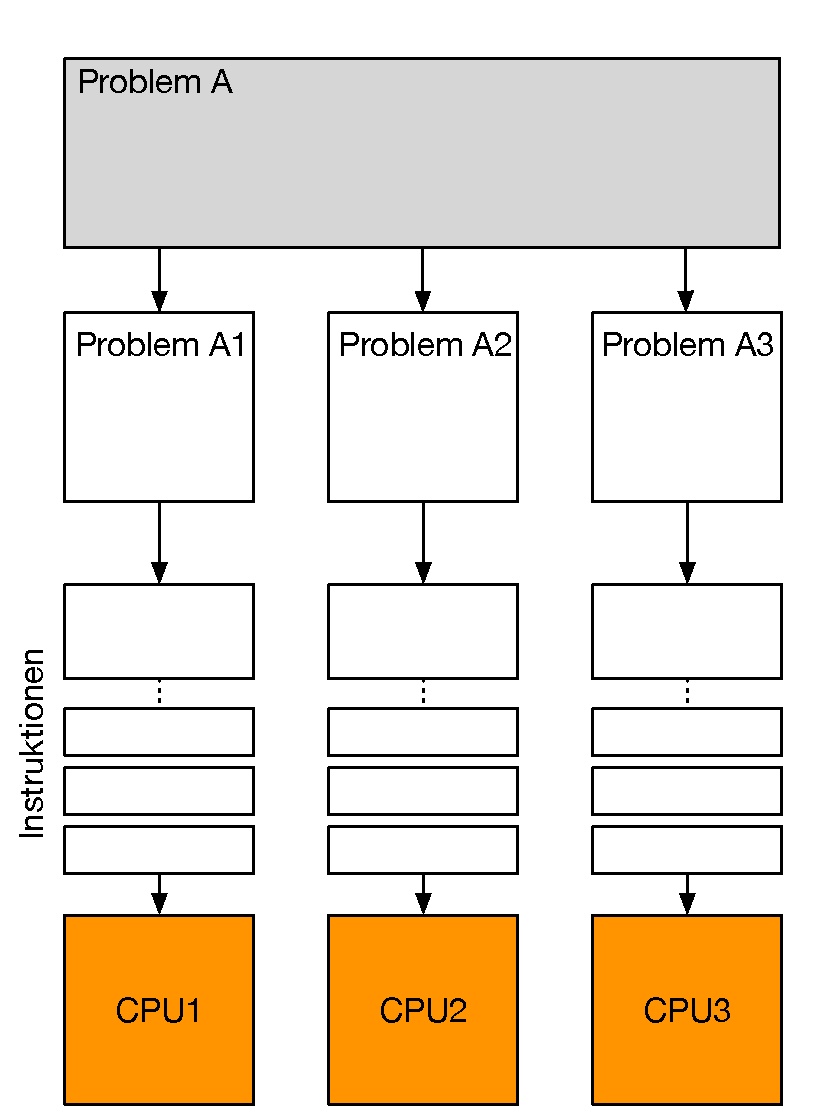
\includegraphics[width=\textwidth]{parallel.pdf}
    \end{columns}
  \end{frame}

  \note[itemize]{
      \item deutscher Begriff schwierig
      \item Aufteilen des Problems in Teilprobleme
      \item Teile können, müssen aber nicht zusammengehörend sein
  }

  \begin{frame}{Nebenläufig}
    \begin{columns}[c]
    \column{.5\textwidth}
      \begin{itemize}
        \item concurrent (engl.)
        \item „Systeme, welche zur gleichen Zeit mehrere \alert{Aufgaben} haben“
        \item muss nicht zwangsläufig parallel sein
        \item Multi-Tasking
      \end{itemize}
    \column{.5\textwidth}
      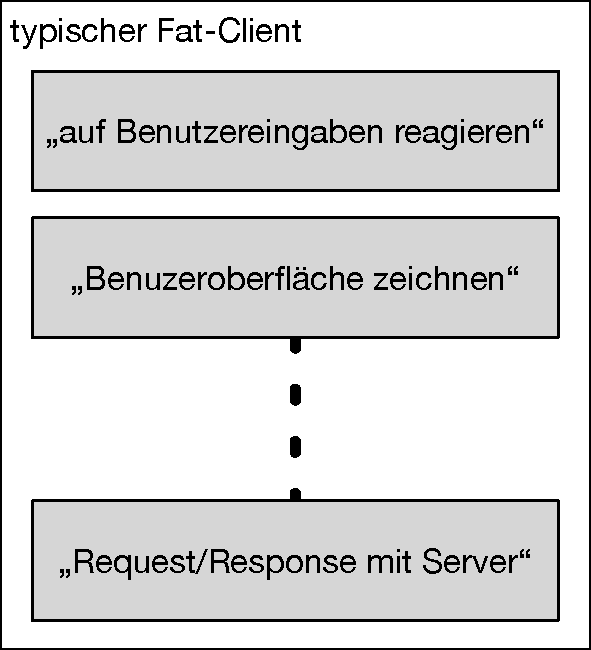
\includegraphics[width=\textwidth]{concurrent.pdf}
    \end{columns}
  \end{frame}
  
  \note[itemize]{
     \item Fokus liegt auf Arichtektur
  }

  \begin{frame}{Rob Pike - „Concurrency Is Not Parallelism“ (1)}
    \begin{itemize}
      \item „Concurrency is about \alert{dealing with} lots of things at once.“
      \item „Parallelism is about \alert{doing} lots of things at once.“
      \item „Concurrency is about structure, parallelism is about execution.“
    \end{itemize}
  \end{frame}

  \note[itemize]{
      \item Rob Pike, Google, Go-Lang
      \item interessanter Talk auf Youtube
  }

  \begin{frame}{Rob Pike - „Concurrency Is Not Parallelism“ (2)}
    
\includegraphics[width=\textwidth]{gophersimple1.pdf}
    \begin{itemize}
      \item sequenziell
    \end{itemize}
  \end{frame}
  
  \note{
    - typischer Aufbau einer App \\
    - Producer/Consumer\\
    - Daten konsolidieren/filtern, Verarbeitung/Transport/Buffer, Weiterverwendung/Ausgabe\\
    - komplett sequenzieller Aufbau, da nur ein worker und alles strikt nacheinander passiert\\
    - problem: ich brauche nur einen gewissen datensatz, dennoch werden alle daten verarbeitet\\
  }

  % \begin{frame}{Rob Pike - „Concurrency Is Not Parallelism“ (3)}
  %   
\includegraphics[width=\textwidth]{gophersimple3.pdf}
  %   \begin{itemize}
  %     \item mehrere Cores, jedoch keine Optimierung
  %   \end{itemize}
  % \end{frame}
  %
  % \note{
  %   - Idee: meine CPU hat mehrere Cores\\
  %   - weitere Cores nutzen persé nichts, da sequenzielle Architektur
  % }

  \begin{frame}{Rob Pike - „Concurrency Is Not Parallelism“ (3)}
    
\includegraphics[width=\textwidth]{gophersimple2.pdf}
    \begin{itemize}
      \item parallel
    \end{itemize}
  \end{frame}
  
  \note{
    - Optimierung einzelner Teile der Applikation\\
    - weitere schritte birgen ähnlich hohen aufwand\\
    - je nach architektur parallelisierung von producer u.U. schwierig\\
  }

  \begin{frame}{Rob Pike - „Concurrency Is Not Parallelism“ (4)}
    
\includegraphics[width=\textwidth]{gophercomplex0.pdf}
    \begin{itemize}
      \item concurrent
    \end{itemize}
  \end{frame}
  
  \note{
    - Nebenläufige Architektur von Anfang an\\
    - d.h. Service-Orientierte Module, die voneinander getrennt funktionieren \\
    - Pro Software-Modul oder Teilsystem eines Moduls kann jeweils ein worker eingesetzt werden. \\
    - architektur kann sehr leicht nach bedarf parallelisiert werden\\
    - nebeneffekt: stabileres System\\
  }

% \section{Threads / Locking}
%   \begin{frame}{Was ist ein Thread?}
%     \begin{columns}[c]
%     \column{.5\textwidth}
%       \begin{itemize}
%         \item Shared Memory
%       \end{itemize}
%     \column{.5\textwidth}
%       \begin{figure}
%         \centering
%         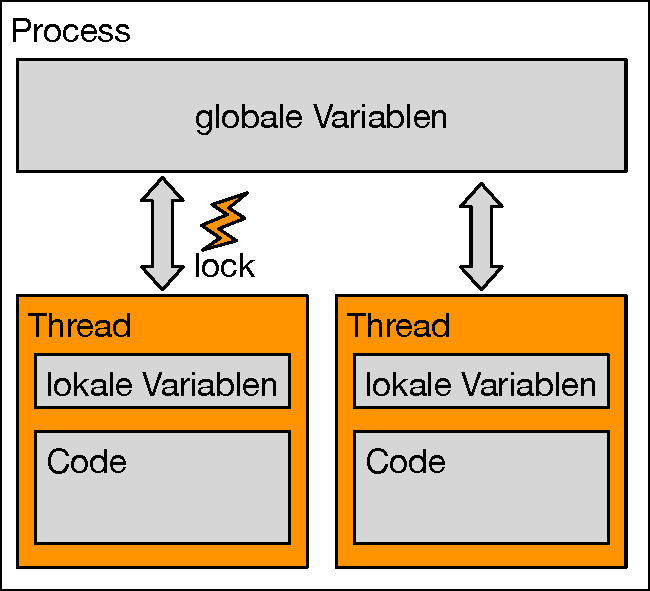
\includegraphics[width=\textwidth]{threads.pdf}
%       \end{figure}
%     \end{columns}
%   \end{frame}
%
%   \begin{frame}{Was ist ein Lock?}
%     \begin{columns}[c]
%     \column{.5\textwidth}
%       \begin{itemize}
%       \item{Dining philosophers problem}
%       \end{itemize}
%     \column{.5\textwidth}
%       \begin{figure}
%         \centering
%         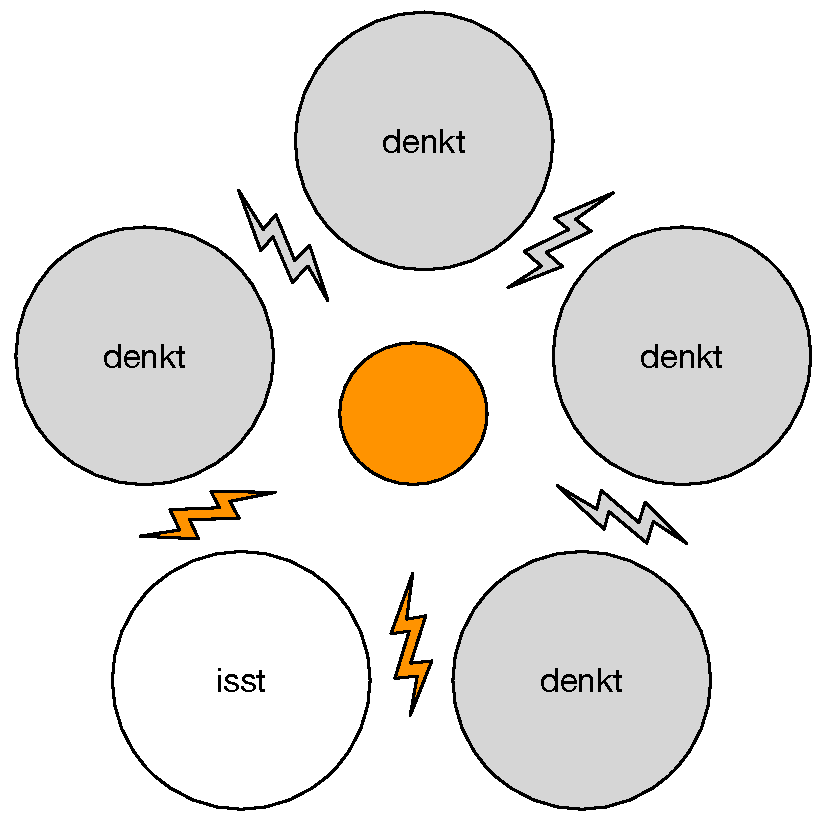
\includegraphics[width=\textwidth]{philosophers_table.pdf}
%       \end{figure}
%     \end{columns}
%   \end{frame}
%
%   \begin{frame}{Häufige Bugs}
%     \begin{columns}[c]
%     \column{.5\textwidth}
%       \textbf{Race-Condition}
%       \begin{itemize}
%         \item ++
%         \item ++
%       \end{itemize}
%     \column{.5\textwidth}
%       \textbf{Deadlock}
%       \begin{itemize}
%         \item --
%         \item --
%       \end{itemize}
%     \end{columns}
%   \end{frame}
%
  % \begin{frame}{Fazit: bisherige Methoden, Motivation FP}
  %   \begin{itemize}
  %     \item nur shared-memory
  %     \item Häufige Bugs bei Threads-Programming (Deadlocks, Race-Conditions,..)
  %     \item Wenige Sprachen helfen Concurrency wirklich leichter zu machen
  %     \item meist keine direkte Unterstützung für reine Parallelisierung
  %     \item Fazit mutability: großen Hierarchien mit  \textit{call-by-reference} führen gerne zu unerwarteten Ergebnissen (bspw. im Browser: DOM-Manipulation)
  %   \end{itemize}
  % \end{frame}
  %
  % \note[itemize]{
  %     \item größtes problem an Thread-ansatz:
  %     \item ohne weitere hilfsmittel kann nebenläufigkeit nur auf einem einzelnen rechner genutzt werden, da threads auf gemeinsamen Speicher/Zustand angewiesen sind
  %     \item Viele Sprachen besitzen threads als feature,
  %     \item wenige Sprachen helfen mit Tooling oder Abstraktion dem Programmierer selbst!
  %     \item führt oft dazu, concurrency zu meiden
  %     \item parallelisierung muss oft mit Threads nachgebaut werden
  % }

  \section{Functional Paradigm 101}
  \begin{frame}{Functional Paradigm 101 (1)}
    \begin{itemize}
      \item immutable // mutable
    \end{itemize}
    \texttt{
    a =  3~~~~~~~a = 3\\
    a += 2~~~~~~~a' = add(a, 2)\\
    a -> 5~~~~~~~a' -> 5
  }
  \end{frame}

  \note{
        1. viele bugs treten durch Veränderung von bestehendem Zustand auf \\
        - in den meisten fällen kann eine Veränderung vermieden werden \\
        - ändert man Zustände, so sollte man besser eine Kopie zurückgeben , anstatt die Referenz zu bearbeiten \\
        - falls gewünscht kann man diese Zustandskopien wie Snapshots in einem Cache betrachten \\
  }

  \begin{frame}{Functional Paradigm 101 (2)}
    \begin{itemize}
      \item no side-effects, deterministisches Verhalten
      \item „pure“, „data-in, data-out“, EVA
      \item functions as first-class citizens
      \item lambdas, callbacks
    \end{itemize}
  \end{frame}

  \note{
        2. ähnlich sollte eine Funktion auch nur diese eine Sache tun, welche man erwartet -> Side-Effects vermeiden\\
    3. Funktionen können als reine daten-transformationen aufgefasst werden \\
    - man bekommt daten, verarbeitet diese und gibt sie verändert zurück. \\
    4. Funktionen sind selbst auch Typen\\
    - d.h. sie können genauso als parameter einer anderen funktion dienen \\
    - sie werden jedoch erst evaluiert, wenn benötigt \\
    5. lamdas sind funktionen, welche inline definiert werden und somit anonym sind \\ 
    - sie haben keinen namen, werden aber oft entweder als callback direkt übergeben oder einer variable zugewiesen \\
  }
  \begin{frame}{Functional Paradigm 101 (3)}
    \begin{itemize}
      \item reine Funktionale Sprachen
    \end{itemize}
  \end{frame}
  \note{
    6. Unterscheidung zwischen Sprachen die Unterstützung für fp bieten \\
    - und solchen die ausschließlich auf den Konzepten und Prinzipien von Funktionalen Sprachen beruhen \\
    - seiten-effekte sind somit niemals möglich\\
    - meistens strikte Typisierung

  }

\section{Elixir}
\begin{frame}{Elixir (1)}
    \begin{columns}[c]
    \column{.5\textwidth}
      \begin{itemize}
        \item 2011: moderne Variante von Erlang\\ (1987, Ericsson)
        \item Beam-VM
        \item lightweight Elixir-Processes
        \item Shared \& Distributed Memory
      \end{itemize}
    \column{.5\textwidth}
      
\includegraphics[width=\textwidth]{elixir.png}
    \end{columns}
  \end{frame}
  
  \note[itemize]{
     \item funktionale Sprache, welche weitestgehend frei von seiten-effekten ist und nutzt eine dynamische typisierung mit typen-interferenz
     \item ob sie nun als reine funktionale bezeichnet werden kann streiten sich einige Fronten
     \item Elixir erweitert Erlang um einige moderne Features wie bspw. metaprogramming und bringt teilweise starke Vereinfachungen bei der Syntax -> ruby
     \item wird zu erlang bytecode compiliert der in beam-vm läuft
     \item Nebenläuffigkeit wird mit Elixir-Processes erreicht, welche jedoch um viele Male leichtgewichtiger sind, als System-Prozesse
     \item je nach anwendungsfall kann man mit elixir sowohl einen gemeinsamen als auch verteilten Zustand nutzen
  }
  \begin{frame}{Elixir (2)}
    \begin{columns}[c]
    \column{.5\textwidth}
      \begin{itemize}
        \item Open Telecom Platform (OTP)
        \item Fault-Tolerant
        \item „Let it crash“
        \item Supervision-Trees
      \end{itemize}
    \column{.5\textwidth}
      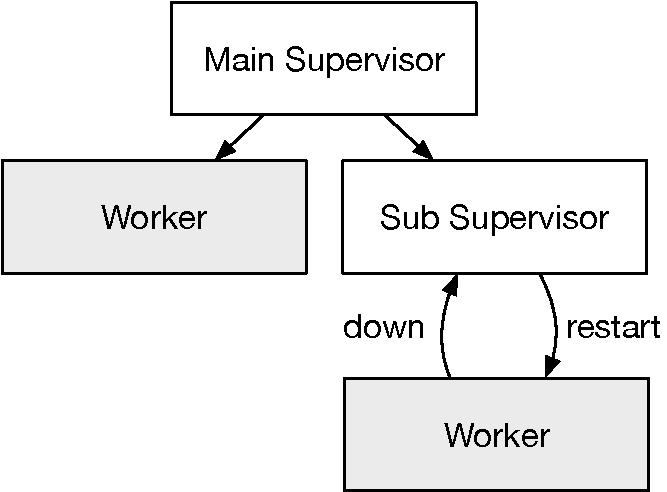
\includegraphics[width=\textwidth]{supervision.pdf}
    \end{columns}
  \end{frame}

  \note[itemize]{
     \item die Fehlerverarbeitung ist interessant gelöst: sollte ein kritischer fehler aufreten, so startet man den prozess einfach neu.
     \item Dies ist durch sogennante provsion-trees möglich
     \item Ein Prozess kann mithilfe des OTP auf einfache art durch einen Supervisor beobachtet werden.
    \item Was im Fehlerfall geschehen soll, entscheidet einer von vielen Algorithmen und es sind damit beliebige schachtelungs-tiefen möglich. bspw. one-for-one
  }

  \begin{frame}{OTP / Actor-Model}
    \begin{columns}[c]
    \column{.5\textwidth}
    \begin{itemize}
      \item Concurrency-Model in Elixir
      \item unabhängige Akteure
      \item Message-Passing
      \item FIFO-Verhalten von \alert{Mailboxes}
      \item Locks werden nicht gebraucht
      \item Alternativen:
        \begin{itemize}
          \item Akka (Java/Scala)
          \item Akka.NET
          \item Pykka (Python)
          \item CAF (C++)
          \item Celluloid (Ruby)
        \end{itemize}
    \end{itemize}
    \column{.5\textwidth}
      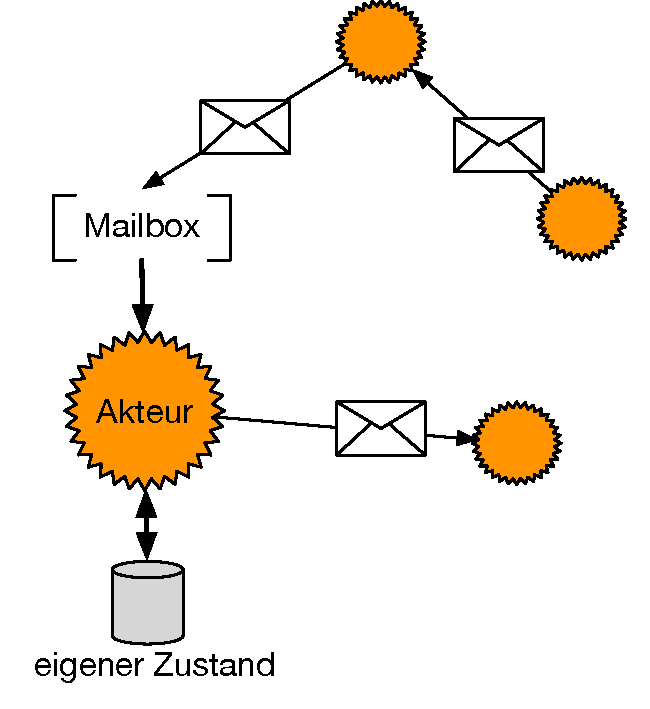
\includegraphics[width=\textwidth]{actors.pdf}
    \end{columns}
  \end{frame}
  
  \note[itemize]{
     \item akteuere können untereinander kommunizieren
     \item besitzen eigenen Zustand, locks werden damit überflüssig
     \item eigener Cache und Persistenz (DB) empfehlenswert
     \item deswegen klar getrennte Services
     \item Messages werden nach reihenfolge des eintreffens verarbeitet
  }

  \begin{frame}{List-Processing in Elixir: map (1)}
    \begin{columns}[c]
    \column{.5\textwidth}
      \begin{itemize}
        \item Iteriert über Collection
        \item Nutzen von transform-function
        \item Ergebnis von gleichem oder verschiedenen Collection-Typ
      \end{itemize}
    \column{.5\textwidth}
    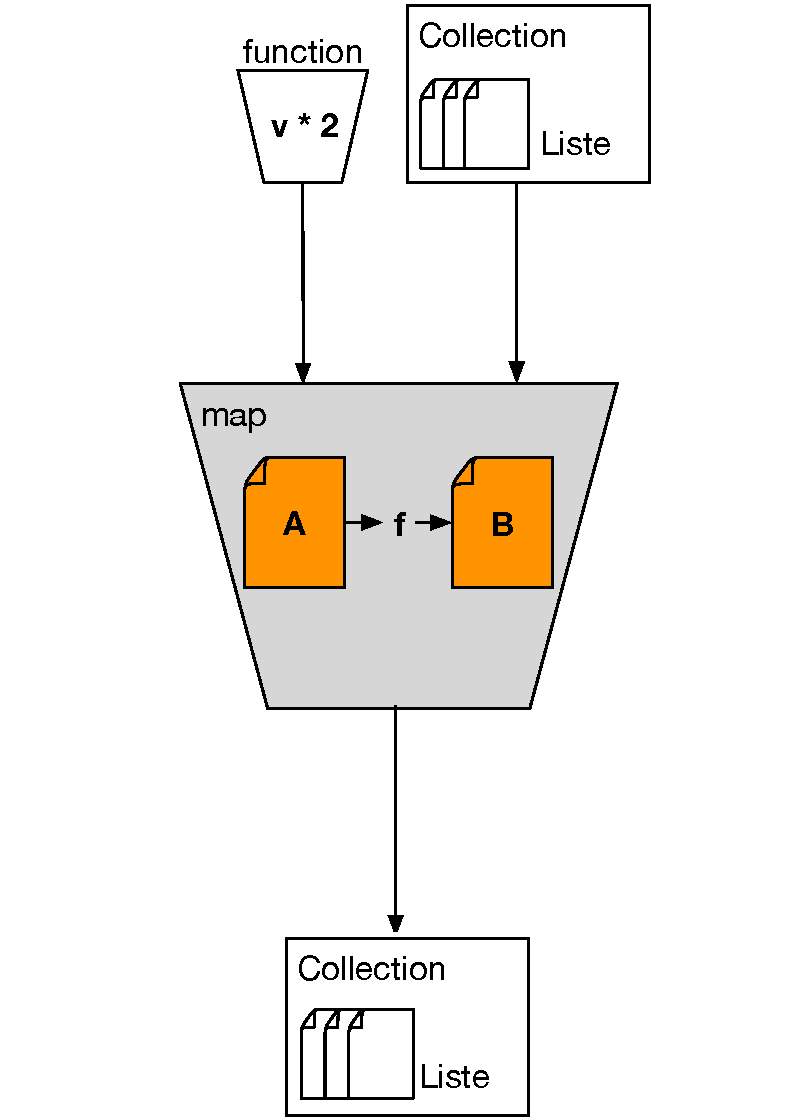
\includegraphics[width=\textwidth]{map.pdf}
    \end{columns}
  \end{frame}
  
  % \note[itemize]{
  %    \item 
  % }

  \begin{frame}{List-Processing in Elixir: map (2)}
    iex = Interactive Elixir \\
    \& = function catch operator
    \begin{itemize}[<+->]
    \item
      \texttt{iex> Enum.map [1, 2, 3], fn x -> x + 1 end} \\
    \item
      \textbf{[2, 3, 4]} \\
    \item
      \texttt{iex> Enum.map [1, 2, 3], \&(\&1 * \&1)} \\
    \item
      \textbf{[1, 4, 9]} \\
    \item
      \texttt{iex> defmodule Math do \\
            ...> def multWithKey(\{k, v\}), do: k * v \\
            ...> end\\
      }
      \textbf{...} \\
    \item
      \texttt{iex> list = Enum.with\_index([1, 2, 3])} \\
    \item
      \textbf{[\{1, 0\}, \{2, 1\}, \{3, 2\}]} \\
    \item
      \texttt{iex> Enum.map list, \&Math.multWithKey/1} \\
    \item
      \textbf{[0, 2, 6]} \\
    \end{itemize}
  \end{frame}

  % \begin{frame}{List-Processing in Elixir: reduce (1)}
  %   \begin{columns}[c]
  %   \column{.5\textwidth}
  %     \begin{itemize}
  %       \item iteriert über Collection
  %       \item Nutzen von aggregate-function und Startwert
  %       \item Mitführen von accumulator
  %       \item „Reduzieren“ der Elemente auf einzelnen gemeinsamen Wert
  %       \item auch \texttt{foldr, foldl} genannt
  %     \end{itemize}
  %   \column{.5\textwidth}
  %   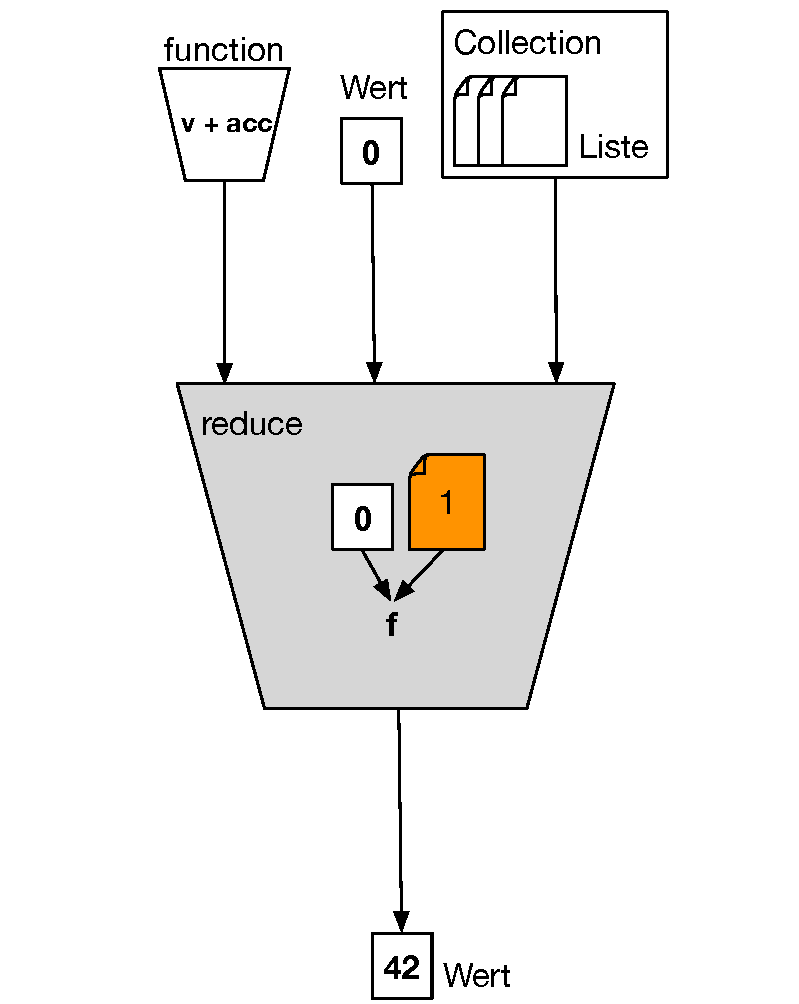
\includegraphics[width=\textwidth]{reduce.pdf}
  %   \end{columns}
  % \end{frame}
  %
  % \note[itemize]{
  %    \item Am anfang ist accumulator=startwert
  % }
  %
  % \begin{frame}{List-Processing in Elixir: reduce (2)}
  %   \begin{itemize}[<+->]
  %     \item \texttt{iex> List.foldl [1, 2, 3, 4], 0, \&(\&1 + \&2)} \\
  %   \item
  %           \textbf{10}
  %         \item \texttt{iex> update\_count = fn word, acc -> \\Map.update acc, String.to\_atom(word), 1, \&(\&1 + 1) end}\\
  %           \textbf{..}
  %         \item \texttt{iex> Enum.reduce(["hello", "my", "name", “is", "hello"], \%\{\}, update\_count)}\\
  %   \item
  %           \textbf{\%\{hello: 2, is: 1, my: 1, name: 1\}}
  %   \end{itemize}
  % \end{frame}

  % \begin{frame}{List-Processing in Elixir: filter (1)}
  %   \begin{columns}[c]
  %   \column{.5\textwidth}
  %     \begin{itemize}
  %       \item iteriert über Collection
  %       \item Nutzen von predicate-function
  %       \item Teilmenge bilden, welche Elemente enthält, welche Anforderung erfüllen
  %     \end{itemize}
  %   \column{.5\textwidth}
  %   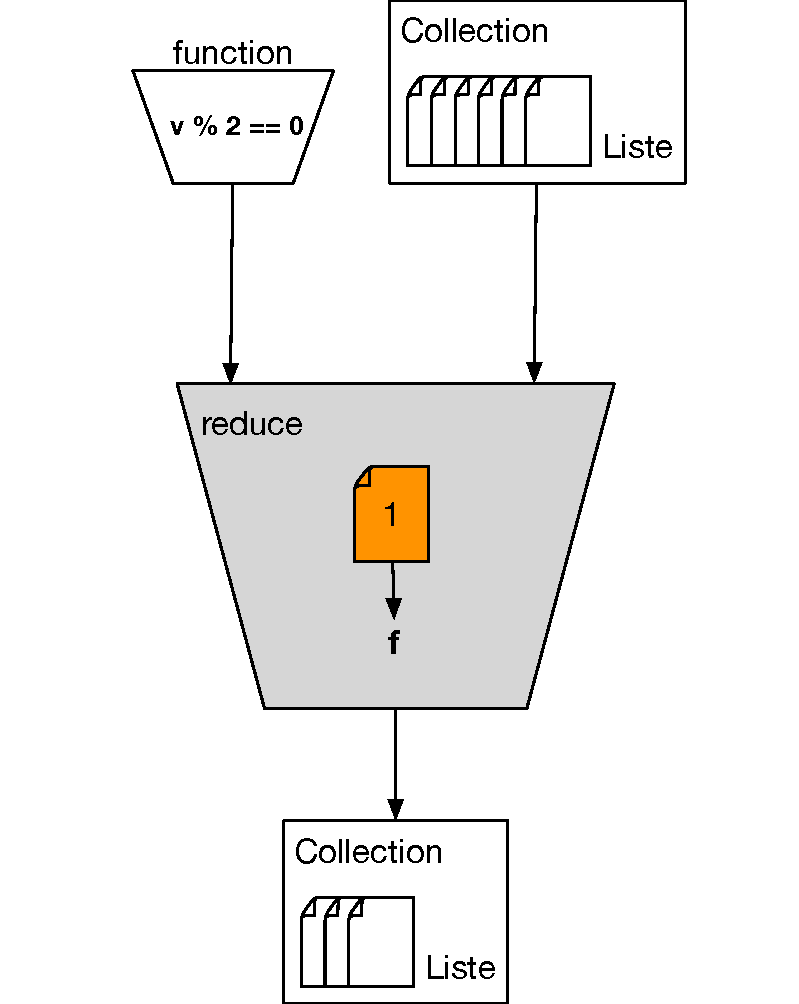
\includegraphics[width=\textwidth]{filter.pdf}
  %   \end{columns}
  % \end{frame}
  %
  % \note[itemize]{
  %    \item 
  % }

  % \begin{frame}{List-Processing in Elixir: filter (2)}
  % \end{frame}

  \begin{frame}{Elixir-Streams (1)}
    \begin{itemize}
      \item große Datenstruktur kann lazy verarbeitet werden
      \item Viele Funktionen aus \texttt{Enum}-Modul 
      \item \texttt{take}: Man erhält immer nur so viele Elemente wie benötigt
      \item function-composition: Jeweiliges Element wird einmalig iteriert und dabei transformiert
      \item siehe Clojure Reducers/Transducers
    \end{itemize}
  \end{frame}

  \note[itemize]{
     \item nicht direkt mit parallelisierung zu tun, jedoch wichtige optimierung dabei
     \item 
  }

  \begin{frame}{Elixir-Streams (2)}
    |> = apply, forward pipe
    \begin{itemize}[<+->]
      \item \texttt{iex> 1..10000 \\|> Stream.map(\&(\&1 * \&1)) \\|> Stream.map(\&(\&1 + \&1))\\ |> Stream.map(\&IO.inspect(\&1))\\ |> Enum.take(10)} \\
      \item 2\\8\\18\\..\\200\\
        \textbf{[2, 8, 18, 32, 50, 72, 98, 128, 162, 200]}
    \end{itemize}
  \end{frame}
  
  \begin{frame}{Elixir-Prozesse erzeugen}
    \texttt{
defmodule Parallel do\\
~~def pmap(collection, fun) do\\
~~~~me = self\\
~~~~collection\\
~~~~|> Enum.map(fn (elem) ->\\
~~~~~~~~spawn fn -> (send me, { self, fun.(elem) }) end\\
~~~~~~~end)\\
~~~~|> Enum.map(fn (pid) ->\\
~~~~~~~~receive do { \^~pid, result } -> result end\\
~~~~~~~end)\\
~~end\\
end\\
    ~\\
    Parallel.pmap 1..1000, \&(\&1 * \&1)\\
  } 
    \begin{itemize}
      \item<2-2> kann ebenso fehleranfällig sein
      \item<2-2> kein Supervisioning, manuelles Error-Handling, Timeouts?
    \end{itemize}
  \end{frame}
  \begin{frame}{OTP-Abstraction: Tasks (1)}
    \begin{itemize}
      \item Task stellt einen simplen Background-Process dar
      \item OTP ist sehr mächtig, jedoch nicht immer eigene Implementierung benötigt
      \item Ein Elixir Process ist häufiger Anwendungsfall
      \item ist in Elixir-Core-Package vorhanden
    \end{itemize}
  \end{frame}
  
  % \note[itemize]{
  %    \item weil otp für Supervisioning in anwendung nutzbar
  % }

  \begin{frame}{OTP-Abstraction: Tasks (2)}
    \texttt{
    defmodule Parallel do\\
    ~~def pmap(collection, func) do\\
    ~~~~collection \\
    ~~~~|> Enum.map(\&(Task.async(fn -> func.(\&1))))\\
    ~~~~|> Enum.map(\&Task.await/1) \\
    ~~end\\
    end\\
    ~\\
    Parallel.pmap 1..1000, \&(\&1 * \&1)\\
  }
    \begin{itemize}
      \item<2-2> noch cleaner als mit \texttt{spawn}
      \item<2-2> möglich Fallstricke sind bereits optimiert
      \item<2-2> weil otp direkt für supervisioning nutzbar
    \end{itemize}
  \end{frame}

\section{Fazit}
  \begin{frame}{Fazit: Functional Programming}
    \begin{columns}[c]
    \column{.5\textwidth}
      \textbf{+~+}
      \begin{itemize}
        \item immutable State eignet sich perfekt für parallel
        \item Higher-Order-Programming: composeability of behaviors
        \item sehr deklarativ 
      \end{itemize}
    \column{.5\textwidth}
      \textbf{-~-}
      \begin{itemize}
        \item Je nachdem steile Lernkurve
        \item Man muss viele bisher eingesetzte Methodiken komplett überdenken
      \end{itemize}
    \end{columns}
  \end{frame}
  
  \note[itemize]{
    \item Je nach Sprache, eher erinnert Programmierung eher an zusammenstellung von Verhalten
    \item HOP, beschäftigt sich genau mit diesem Thema
    \item Art und Abfolge der Anweisung kann genau und deklarativ bestimmt werden
    \item Bei Nutzen des OTP nebenläufiges und verteiletes System von hause aus
      \item Häufige Bugs bei Threads-Programming (Deadlocks, Race-Conditions,..) werden einfach umgangen
      \item Wenige Sprachen helfen Concurrency wirklich leichter zu machen
      \item meist keine direkte Unterstützung für reine Parallelisierung
  }

  % \begin{frame}{Functional Style in Imperative Languages}
  % \end{frame}
  %
  % \note[itemize]{
  %    \item 
  % }
\end{document}
